\chapter{Windows development}

\section{Creation of the work environment}

In the previous chapter we used VirtualBox to create a Linux environment in which we developed various programs. 
Now we have to create another environment, this time for Windows, as we will study the state of the art of eBPF on this latest operating system.

Remembering that the computer on which the process was carried out has Windows 11 as its operating system, for this purpose we used the \textit{Hyper-V Console Manager}, a native Windows feature, to create a separate Windows 11 virtual machine.
\textit{Hyper-V} is a type 1 (or bare-metal) virtualization software, also known as a \textit{Virtual Machine Monitor} (\textit{VMM}), which runs directly on the physical hardware without the need for an underlying host operating system. 
The illustrative representation of the architecture just described is depicted in Figure \ref{fig:type_1_hypervisor}.
As the core software responsible for managing virtual machines and allocating hardware resources to each VM, Hyper-V ensures better security and resource utilization by isolating each VM from others and the host OS. 
With direct access to the physical hardware, it efficiently allocates resources, resulting in improved performance, isolation and scalability compared to type 2 hypervisors like VirtualBox.

\begin{figure}[h]
	\centering
	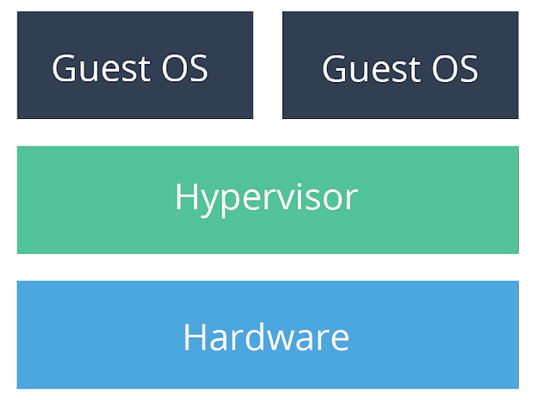
\includegraphics[width=0.7\linewidth]{images/Technologies/type_1_hypervisor.png}
	\caption{Type 1 (or bare metal) hypervisor architecture \cite{HypervisorsArchitectures}.}
	\label{fig:type_1_hypervisor}
\end{figure}

The greatest benefits of hypervisors are their robustness and scalability, enabling the efficient virtualization of large-scale applications and services.
However, the choice of creating a virtual machine using the Hyper-V Console Manager was dictated by two other reasons:

\begin{itemize}
	\item 
		The setup instructions described on the \textit{ebpf-for-windows} GitHub repository tell the user to install a Windows VM \cite{VMSetup};
	\item 
		The so created isolated Windows 11 development environment provided a controlled space for testing and optimizing eBPF programs on the Windows platform.
		In fact, if anything goes wrong in this environment, we just delete the virtual machine and create a new one, while if something bad happens on our host machine, we could break our computer.
\end{itemize}

We are going to talk about the eBPF installation on Windows later: for now, besides the fact that that he virtual machine was configured with adequate resources to support development tasks effectively, the only thing worth noting is that during the quick creation of the virtual machine the option of ``Windows 11 dev environment'' must be selected (the tutorial tells to choose the ``Windows 10 dev environment'', but Windows 11 works as well).  


\section{ebpf for Windows}

% https://microsoft.github.io/ebpf-for-windows/ -> MANUAL PAGE

% https://github.com/Microsoft/ebpf-for-windows/ 

\section{windows ebpf starter}

% https://github.com/SubconsciousCompute/windows-ebpf-starter